%final report
%\documentclass{FRIreport}

%internal report
%\documentclass[internal]{FRIreport}

%seminar report
\documentclass[seminar]{FRIreport}

% AMS fonts required
\usepackage{iopams}  

% package to include graphics in ps, eps or png format
\usepackage{graphicx}
\usepackage{epstopdf}
% the graphics path
\graphicspath{{img/}}

% define equation referencing
\newcommand{\eqref}[1]{(\ref{#1})}

% define figure referencing
\newcommand{\figref}[1]{Fig.~\ref{#1}}

% define real numbers symbol
\newcommand{\Rset}{\ensuremath{\mathbb{R}}} 
\newcommand{\R}{\Rset} 
% define natural numbers symbol
\newcommand{\Nset}{\ensuremath{\mathbb{N}}} 
\newcommand{\N}{\Nset} 
% define euclidean vector space symbol
\newcommand{\Eset}{\ensuremath{\mathbb{E}}} 
\newcommand{\E}{\Eset} 

\newcommand{\imp}[1]{{\color{P654M}#1\normalcolor}}

%main
\begin{document}

\title{qdCAD: the quantum-dot engine}

\author[P {Pe�ar} \etal]{{Primo�} {Pe�ar}, Miha Mo�kon, Iztok Lebar Bajec}

\address{Group 1}

\begin{abstract}
A short abstract is always usefull for the reader to quickly evaluate if the paper is intersting to him or not. The abstract should be written in a manner to summarize the paper content and attract the reader.

\Keywords{quantum-dot cellular automata, modelling and simulation}
\end{abstract}



%
%%
\section{Introduction}
%
The Hamiltonian ... Ternary logic done with ternary quantum-dot cell \cite{lebar_bajec:2005c,lebar_bajec:2006a,lebar_bajec:2006b}.

%
%%
\section{Methods}
%
present the employed methods

%
\subsection{Method 1}
give overview of method 

%
%%
\section{Results and Discussion}
%
show some results like \figref{fig.Df} and discuss them
%
\begin{figure}[htb]
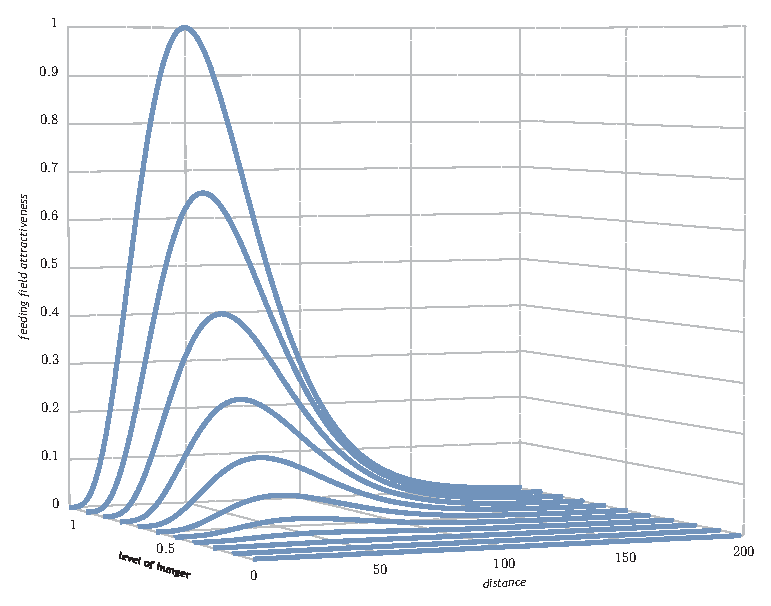
\includegraphics{figDf.eps}
\caption{Use figures to show results.}
\label{fig.Df}
\end{figure}
%

%
%%
\section{Conclusion}
%
finish by presenting some future research directions

%
%%
\References
%
\bibliographystyle{elsart-num}
\bibliography{sample}

\end{document}
